\documentclass{beamer}
\usepackage{amsfonts}
\usepackage{amssymb}
\usepackage{amsmath}
\usepackage{amsthm}
\usepackage{mathtools}
\usepackage{graphicx}

\usepackage{sansmathaccent}

\DeclareMathOperator*{\argmin}{arg\,min}
 
\usepackage[utf8]{inputenc}
\usetheme[compress]{Berlin}
\usecolortheme{beaver}
 
\title{Random Barrier Avoidance Using Risk-Constrained MDPs}
\author{Lucas Berry}
\institute{Comp 767}
\date{April 20th, 2017}

\begin{document}
\maketitle
\begin{frame}
	\frametitle{Introduction}
	In many applications one is concerned with in maximizing expected return while also mitigating risk. This gives rise to the study of risk measures and risk averse policy search. The objects of interest are rare risky events.
	\pause
	\begin{center}
	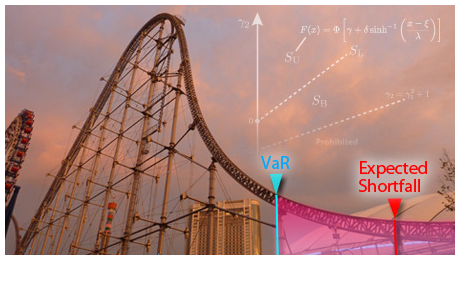
\includegraphics[scale=.4]{expected-shortfall}     
	\end{center}	
\end{frame}
\begin{frame}
	\frametitle{CVaR and VaR}
	Two commonly used risk measures are value at risk (VaR) and conditional value at risk (CVaR) also known as expected shorfall (ES) and average value at risk (AVaR). VaR and CVaR are defined as,
	\begin{align*}
		VaR_{\alpha}(X) &:= inf\lbrace{x | P(X\leq x)\geq\alpha\rbrace},\\
		CVaR_{\alpha}(X) &:= E\left[X|X\geq VaR_{\alpha}(X)\right]. 
	\end{align*}
	\pause
	CVaR can be rewritten in a more useful way for optimization,
	\begin{align*}
	CVaR_{\alpha}(X) = \min_{\nu \in \mathbb{R}}\left\lbrace \nu + \frac{1}{1-\alpha}E\left[(X-\nu)^+\right]\right\rbrace,
	\end{align*}
	where $(x)^+ = \max(0,x)$.  
\end{frame}
\begin{frame}
	\frametitle{Risk Constrained MDPs}
	In Chow et. al [2015] the authors derive 5 policy gradient algorithms to solve risk sensitive MDPs constrained by $CVaR$ and $VaR$. The optimization problem is rephrased as,
	\begin{displaymath}
		\min_{\theta} V^{\theta}(s_0) \qquad \text{subject to} \qquad CVaR_{\alpha}(\sum_{k=1}^{T}\gamma^kR_k)\leq \beta,
	\end{displaymath}
	\pause
	and
	\begin{displaymath}
		\min_{\theta} V^{\theta}(s_0) \qquad \text{subject to} \qquad P(\sum_{k=1}^{T}\gamma^kR_k\geq\beta)\leq 1-\alpha.
	\end{displaymath}
	Please note $\alpha \in (0,1)$, $\beta \in \mathbb{R}$ and the constraint in (2) is another way of writing VaR. Also let $G_T=\sum_{k=1}^{T}\gamma^kR_k$. 
\end{frame}
\begin{frame}
	\frametitle{Finding a Solution}
	To solve (1) Chow et. al [2015] follows the Lagrangian relaxation procedure described in Chapter 3 of Bertsekas (1999) yielding,
	\begin{displaymath}
	\max_{\lambda \geq 0}\min_{\theta, \nu}\left[L(\nu,\theta,\lambda):=V^{\theta}(s_0)+\lambda\left(H_{\alpha}\left(G_T,\nu\right)-\beta\right)\right],
	\end{displaymath}
	where
	\begin{displaymath}
	H_{\alpha}(X,\nu) := \nu + \frac{1}{1-\alpha}E\left[(X-\nu)^+\right].
	\end{displaymath}
\end{frame}
\begin{frame}
	\frametitle{Gradients}
	Computing the necessary gradients gives
	\begin{align*}
	&\nabla_{\theta}L(\nu,\theta,\lambda)=\nabla_{\theta}V^{\theta}(s_0)+\frac{\lambda}{1-\alpha}\nabla_{\theta}E\left[\left(G_T-\nu\right)^+\right],\\
	&\partial_{\nu}L(\nu,\theta,\lambda)=\lambda\left(1+\frac{1}{1-\alpha}\partial_{\nu}E\left[\left(G_T-\nu\right)^+\right]\right),\\
	&\nabla_{\lambda}L(\nu,\theta,\lambda)= \nu+\frac{1}{1-\alpha}E\left[\left(G_T-\nu\right)^+\right].
	\end{align*}
\end{frame}
\begin{frame}
	\frametitle{Monte-Carlo}
		 $\nu$ \textbf{Update}:\\
		  $ \nu_{k+1}=\Gamma_{\mathcal{N}}\left[ \nu_k-\zeta_3(k)\left(\lambda_k-\frac{\lambda_k}{(1-\alpha)N} \sum\limits_{j=1}^N\mathbf{1}\{G_T(j,k) \geq \nu_k\}\right)\right] $\\
		 $\theta$ \textbf{Update}:
				\begin{align}
				&\theta_{k+1}  =\Gamma_{\Theta}\bigg[ \theta_k-\zeta_2(k)\bigg(\frac{1}{N}\sum\limits_{j=1}^N \nabla_{\theta}\log \mathbb{P}_{\theta}(\xi_{j,k})\big| _{\theta=\theta_k}G_T(j,k)+ \notag\\
				&\frac{\lambda_k}{(1-\alpha)N} \sum\limits_{j=1}^N \nabla_{\theta}\log \mathbb{P}_{\theta}(\xi_{j,k})\big| _{\theta=\theta_k} (G_T(j,k) - \nu_k \})\mathbf{1}\{G_T(j,k) \geq \nu_k\}\bigg)\bigg] \notag
				\end{align} 
\end{frame}
\begin{frame}
	\frametitle{Monte-Carlo}
	$\lambda$ \textbf{Update}:
	\begin{align}
	\lambda_{k+1}&=\Gamma_{\Lambda}\bigg[ \lambda_k-\zeta_1(k)\bigg(\nu_k - \beta\\
	& + \frac{1}{(1-\alpha)N}\sum\limits_{j=1}^N(G_T(j,k) - \nu_k )\mathbf{1}\{G_T(j,k) \geq \nu_k\}\bigg)\bigg] \notag
	\end{align}
\end{frame}
\begin{frame}
	\frametitle{Random Barriers}
	In Chow et. al [2015] they used their algorithm for a financial mathematics problem. I wanted to apply it to a robotics problem.
	\begin{center}
	 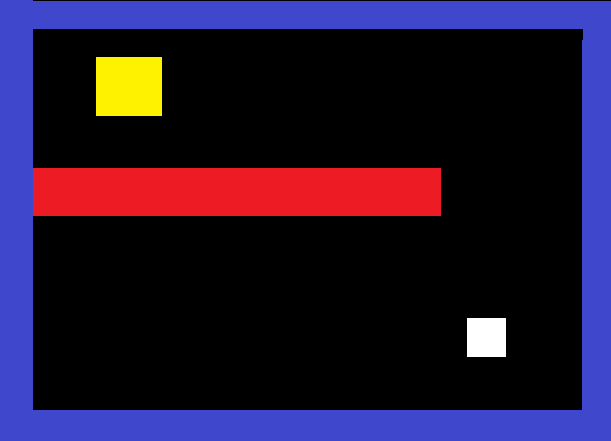
\includegraphics[scale=.4]{Random_barrier}
	\end{center} 
\end{frame}


\end{document}